\section{Theoretical Background}
% \addcontentsline{toc}{section}{Theoretical Background}
\fancyhead[R]{Theoretical Background}

\subsection{Principles of Enzymology}
\label{sec:Principles of Enzymology}

Enzymology is the study of enzymes, which are biological catalysts that accelerate biochemical reactions in living organisms. These macromolecules are essential for various cellular processes, including metabolism, DNA replication, and signal transduction. The understanding of enzyme structure, function, and kinetics is crucial for developing applications in biotechnology, medicine, and environmental science. \footcite{robinsonEnzymesPrinciplesBiotechnological2015}

\subsubsection{Enzyme Classification and Function}
\label{sec:Enzyme Classification and Function}

Enzymes are classified based on the reactions they catalyze, following a system established by the Enzyme Commission (EC). This classification system groups enzymes into six main classes, each with specific types of reactions they facilitate:

\begin{compactenum}
    \item \textbf{Oxidoreductases:} These enzymes catalyze oxidation-reduction reactions, where the transfer of electrons occurs between molecules. Examples include dehydrogenases and oxidases.
    
    \item \textbf{Transferases:} These enzymes transfer functional groups from one molecule to another. Examples include kinases, which transfer phosphate groups.
    
    \item \textbf{Hydrolases:} These enzymes catalyze the hydrolysis of various bonds, including ester, glycosidic, peptide, and others. Examples include proteases and lipases.
    
    \item \textbf{Lyases:} These enzymes add or remove groups to form double bonds, without hydrolysis or oxidation. Examples include decarboxylases and dehydratases.
    
    \item \textbf{Isomerases:} These enzymes catalyze the rearrangement of atoms within a molecule, leading to isomerization. Examples include racemases and epimerases.
    
    \item \textbf{Ligases:} These enzymes catalyze the joining of two molecules with the simultaneous hydrolysis of a diphosphate bond in ATP or a similar triphosphate. Examples include synthetases and carboxylases.
    
\end{compactenum}

-- Überleitung finden --
The three-dimensional (3D) structure of enzymes is fundamental to their function. Enzymes are composed of one or more polypeptide chains that fold into specific shapes to form the active site. The active site is where substrate molecules bind and undergo a chemical reaction. The enzyme structure serves as a scaffold to support and correctly position the active site for optimal catalytic activity. 

\begin{figure}[hbt]
    \centering
    \begin{minipage}[t]{.9\textwidth}
    \caption{Organisation of enzyme structure and lysozyme example.}
    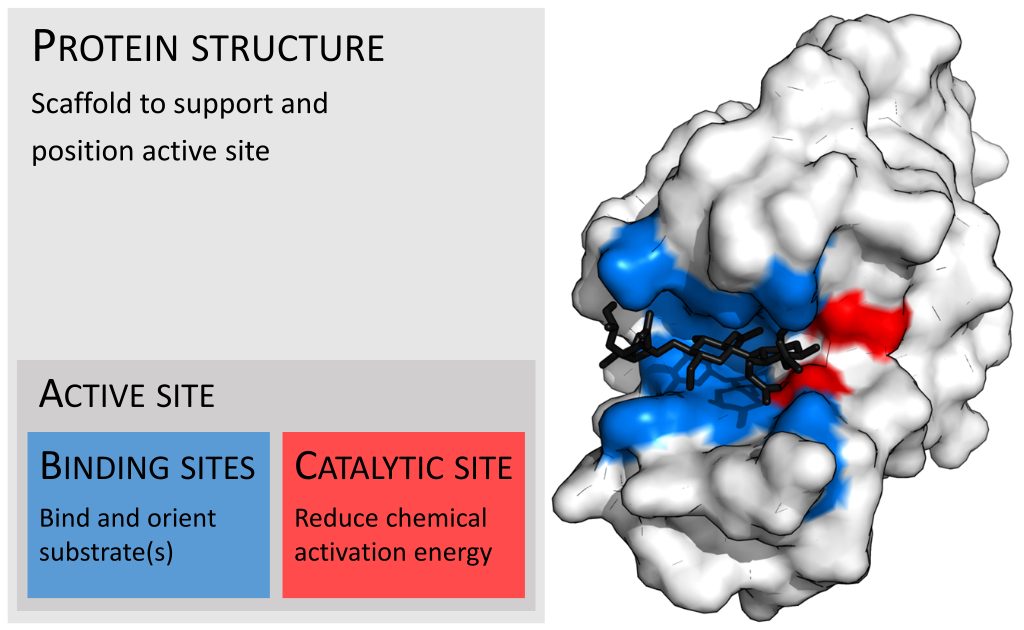
\includegraphics[width=1\textwidth]{img/EnzymeStructure.svg.png}\\
    \source{Thomas Shafee, CC BY 4.0 via Wikimedia Commons}
    \label{fig:EnzymeStructure}
    \end{minipage}
\end{figure}

\begin{itemize}
    \item \textbf{Protein Structure:} The overall structure of the enzyme provides the framework that supports and positions the active site. This structure is critical for the enzyme's stability and functionality. The enzyme's polypeptide chains fold into a unique 3D shape, creating a specific environment for the active site.
    \item \textbf{Active Site:} The active site includes two critical regions: binding sites and the catalytic site. The binding sites (highlighted in blue) are regions where substrates bind to the enzyme. These sites ensure that the substrates are properly oriented for the reaction. The catalytic site (highlighted in red) is the region where the chemical reaction occurs. The catalytic site often contains amino acids with specific functional groups that participate directly in the reaction, reducing the activation energy required for the reaction to proceed.
\end{itemize}

The precise arrangement of amino acids in the active site allows enzymes to be highly specific for their substrates, facilitating efficient catalysis. This specificity is a key feature that enables enzymes to perform their roles in various biochemical pathways with high precision.

A study by Veselovsky et al. (2001) emphasizes the importance of visualizing active site structures, even for enzymes with unknown 3D structures. By analyzing enzyme interactions with reversible competitive inhibitors and molding the substrate-binding region, researchers can predict the shape and dimensions of the active site. This approach has been validated by comparing it with known enzyme-inhibitor complexes, demonstrating its utility in understanding enzyme function and aiding in the search for new ligands.\footcite{veselovskyApproachVisualizationActive2001}

\subsubsection{Role of Enzymes in Biodegradation}
\label{sec:Role of Enzymes in Biodegradation}

Enzymes play a crucial role in the biodegradation of pollutants, including pesticides. The process involves the breakdown of complex organic molecules into simpler, less toxic forms. This degradation is essential for reducing environmental pollution and mitigating the adverse effects of hazardous chemicals.

Hydrolytic Enzymes: Hydrolytic enzymes, such as esterases and amidases, catalyze the cleavage of ester and amide bonds in pesticide molecules. This hydrolysis results in the formation of smaller, more water-soluble compounds that are easier to further degrade and eliminate. For example, microbial esterases can hydrolyze organophosphate insecticides, significantly accelerating their breakdown. \footcite{munneckeEnzymaticHydrolysisOrganophosphate1976a}

Oxidative Enzymes: Oxidative enzymes, such as cytochrome P450 monooxygenases, introduce oxygen atoms into the pesticide molecules, increasing their solubility and reactivity. This oxidation process often converts the pesticides into less harmful substances or intermediates that can be further degraded by other enzymes. The cytochrome P450 enzymes are particularly versatile, capable of metabolizing a wide range of xenobiotics, including pesticides. \footcite{belloTheoreticalApproachMechanism2000}

Reductive Enzymes: Reductive enzymes, including reductases, catalyze the reduction of pesticides, often by adding electrons and hydrogen atoms to the molecules. This reduction can break down complex structures and facilitate the conversion of pesticides into simpler, less toxic forms. Reductive dehalogenases, for instance, play a significant role in the degradation of halogenated organic compounds.

The integration of enzymatic biodegradation with deep learning models can enhance the prediction and analysis of these processes. By using deep learning to analyze enzyme-substrate interactions and their corresponding (EC) classification, we can develop more accurate and efficient bioremediation strategies.

\subsection{Fundamentals of Machine Learning and Deep Learning}
\label{sec:Fundamentals of Deep Learning}

Machine Learning and Deep Learning are two powerful techniques in the realm of machine learning, each offering unique strengths for different types of data and prediction tasks. While deep learning excels at handling unstructured data and automatically extracting features, Machine Learning e.g. Random Forest is known for its robustness, interpretability, and effectiveness in handling structured data with high-dimensional features. This section focuses on the use of Random Forest for sequence-based predictions, particularly in the context of predicting enzyme classes based on protein sequences.

\subsubsection{Introduction to Deep Learning}
\label{sec:Introduction to Deep Learning}

Deep learning has dramatically transformed various fields by enabling the analysis and interpretation of complex datasets. Unlike traditional machine learning methods, which often require manual feature extraction, deep learning models can automatically learn relevant features from raw data. This capability is largely due to the hierarchical structure of neural networks, which can capture multiple levels of abstraction.

A deep neural network is composed of an input layer, multiple hidden layers, and an output layer. Each layer consists of nodes (neurons) that are interconnected with nodes from the previous and next layers. The strength of these connections is determined by weights, which are adjusted during the training process to minimize prediction error. The training is typically performed using a variant of stochastic gradient descent (SGD) and backpropagation, a method for computing the gradient of the loss function with respect to each weight. \footcite{bishopPatternRecognitionMachine2006}

The following image illustrates the basic structure of a deep neural network:

\begin{figure}[hbt]
    \centering
    \begin{minipage}[t]{.9\textwidth}
    \caption{Diagram of a multi-layer feedforward artificial neural network.}
    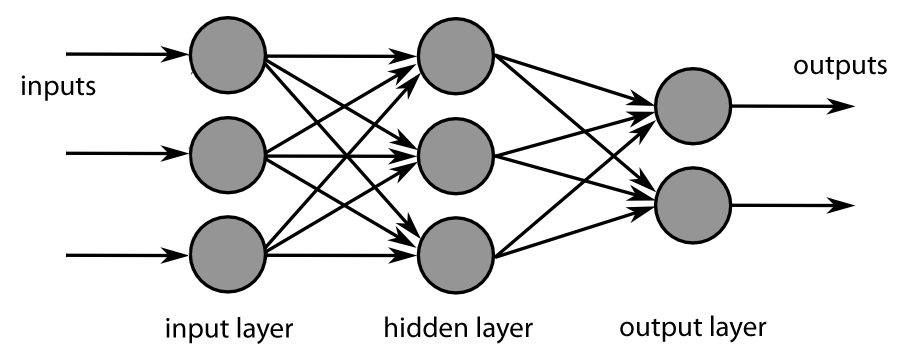
\includegraphics[width=1\textwidth]{img/MultiLayer Neural Network Bigger.png}\\
    \source{Chrislbderivative work, CC BY-SA 3.0 via Wikimedia Commons}
    \label{fig:feedforward_neural_network}
    \end{minipage}
\end{figure}

In this structure, the input layer receives raw data. This data is then processed through one or more hidden layers, where the neurons apply weights and activation functions to capture complex patterns and features. Finally, the processed information reaches the output layer, where the final prediction or classification is made.

Deep learning is particularly effective for problems involving high-dimensional and unstructured data, such as images, audio, and text. Its ability to automatically extract and learn complex features from raw data makes it superior to traditional machine learning methods, which often rely on manually engineered features that may not capture the full complexity of the data.

\subsubsection{Fundamentals of Ligand Binding Site Prediction}
\label{sec:Fundamentals of Ligand Binding Site Prediction}

As mentioned earlier, enzymes interact with substrates at specific binding sites, where the catalytic reactions occur. Predicting these ligand-binding sites is crucial for understanding enzyme function and substrate specificity. Several computational methods have been developed to predict ligand-binding sites from protein structures, including geometric, physicochemical, and machine learning-based approaches.

P2Rank is a machine learning-based tool designed for the rapid and accurate prediction of ligand binding sites from protein structures. It employs a combination of geometric and physicochemical descriptors to analyze protein structures and predict the locations of potential binding sites. P2Rank uses a random forest algorithm, an ensemble learning method that constructs multiple decision trees during training and outputs the mode of the classes (classification) or mean prediction (regression) of the individual trees.

The tool focuses on the interactive parts of enzymes, particularly the ligand-binding sites and the specific amino acids involved. This detailed analysis allows for accurate predictions of enzyme classes and their associated degradation pathways. P2Rank's ability to quickly and accurately predict binding sites makes it a valuable tool for drug discovery and environmental bioremediation applications.

The following image illustrates the workflow of P2Rank, highlighting the process of predicting ligand binding sites from protein structures:

-- P2Rank Workflow --

P2Rank's approach can significantly enhance the accuracy of predicting enzyme-mediated degradation of pesticides by providing detailed insights into the binding interactions at the molecular level. This integration of deep learning and enzyme analysis forms a robust framework for developing bioremediation strategies and understanding the environmental fate of various pollutants. \footcite{krivakP2RankMachineLearning2018}

\subsubsection{Sequence-Based Machine Learning}
\label{sec:Sequence-Based Machine Learning}

In this thesis context, sequence-based machine learning refers to the use of protein sequences as input data for predicting enzyme classes. The sequences are typically represented as strings of amino acids, with each amino acid corresponding to a specific position in the sequence. Machine learning models, such as Random Forest, can analyze these sequences and extract relevant features to predict the enzyme class. This approach uses a Random Forest algorithm, an ensemble learning method that operates by constructing a multitude of decision trees during training and outputting the mode of the classes (classification) or mean prediction (regression) of the individual trees. This method was introduced by Leo Breiman in 2001 and has since become a staple in bioinformatics and other scientific fields due to its versatility and performance. \footcite{breimanRandomForests2001}

The workflow for sequence-based machine learning involves the following steps:

\begin{enumerate}
    \item \textbf{Feature Extraction}: The sequence data, such as amino acid sequences, are first transformed into numerical features. This can include k-mer counts, physicochemical properties of amino acids, and other sequence-derived features.
    \item \textbf{Model Training}: These features are used to train the Random Forest model, which learns to associate specific patterns in the sequence data with enzyme classes.
    \item \textbf{Prediction}: Once trained, the model can predict the enzyme class of new, unseen sequences.
\end{enumerate}

A significant advantage of using Random Forest in this context is its ability to handle complex interaction structures and high-dimensional feature spaces, which are common in biological sequence data. \footcite{diaz-uriarteGeneSelectionClassification2006}

In the context of this study, deep learning techniques are utilized for predicting ligand-binding sites, which are crucial for understanding protein function and interaction with other molecules. Tools like p2rank can be used to predict these binding sites from protein structures, providing the base for a Random Forest model to predict the enzyme class based on the identified ligand-binding sites. This combined approach leverages the strengths of deep learning for feature extraction and Random Forest for classification, enhancing the accuracy and reliability of enzyme class predictions

\subsubsection{Evaluation of Machine Learning Models}
\label{sec:Evaluation of Machine Learning Models}

Evaluating deep learning models involves several metrics and techniques to ensure their accuracy and generalizability. This is essential not only for validating the model’s performance but also for comparing it against other models. Using independent datasets for benchmarking is crucial to demonstrate the model's robustness and applicability to real-world scenarios. Several key metrics are commonly used to evaluate deep learning models:

\begin{enumerate}
    \item \textbf{Accuracy:} The ratio of correctly predicted instances to the total instances. It provides a straightforward measure of performance but can be misleading if the data is imbalanced. \footcite{AccuracyPrecision2024}
    \item \textbf{Precision:} The ratio of true positive predictions to the total predicted positives. Precision is crucial when the cost of false positives is high.
    \item \textbf{Recall (Sensitivity):} The ratio of true positive predictions to the total actual positives. Recall is important when the cost of false negatives is high. \footcite{PrecisionRecall2024}
    \item \textbf{F1-Score:} The harmonic mean of precision and recall, providing a single metric that balances both. It is useful when there is an uneven class distribution. \footcite{Fscore2024}
    \item \textbf{ROC-AUC (Receiver Operating Characteristic - Area Under Curve):} A performance measurement for classification problems at various threshold settings. It tells how much the model is capable of distinguishing between classes. \footcite{ReceiverOperatingCharacteristic2024}
\end{enumerate}

Using these metrics, the performance of deep learning models can be tested on independent datasets. This is critical for ensuring that the models are not just overfitting to the training data but can generalize well to new, unseen data.

In the context of comparing different models, these metrics allow for a standardized evaluation process. By applying the models to benchmark datasets, researches can objectively measure and compare their performance. For instance, in the case of predicting enzyme-mediated pesticide degradation, using independent datasets ensures that the model’s predictions are reliable and can be generalized across various enzyme and pesticide types.

Model evaluation is essential for several reasons: \footcite{emmert-streibIntroductoryReviewDeep2020}

\begin{enumerate}
    \item \textbf{Validation of Model Performance:} Ensuring that the model performs well not just on the training data but also on new, unseen data. This is crucial for the model's reliability and applicability in real-world scenarios.
    \item \textbf{Comparison with Other Models:} By using standardized evaluation metrics and independent datasets, we can objectively compare the performance of different models. This helps in identifying the most effective model for a given task.
    \item \textbf{Identification of Overfitting:} Evaluating the model on independent datasets helps in identifying overfitting, where the model performs well on training data but poorly on new data. Regularization techniques and cross-validation can be used to mitigate this issue.
    \item \textbf{Continuous Improvement:} Regular evaluation allows for continuous monitoring and improvement of the model. Feedback from evaluation metrics can guide further tuning and optimization of the model.
    \item \textbf{Transparency and Trust:} Providing clear and objective evaluation metrics builds trust with stakeholders and users of the model. It ensures that the model’s predictions are transparent and can be trusted for decision-making.
\end{enumerate}

Using benchmark datasets and standardized metrics is a best practice in machine learning and deep learning. It ensures that the models are robust, reliable, and ready for deployment in practical applications. In the context of environmental science and bioremediation, such rigorous evaluation is crucial for developing effective and reliable models for predicting pesticide degradation and other complex processes.